\chapter{Learning methods and design choices}
\section[Learning method]{Learning methods \hfill \small \normalfont\textit{by Matthias Hericks}}

\subsection{Generalized policy iteration}

In their most abstract form, all of the reinforcement learning methods we deployed during this project can be described as \emph{generalized policy iteration}. The key components of generalized policy iteration are two interacting processes. The \emph{policy iteration} process, makes a value function $v$ or action-value function $q$ increasingly consistent with the policy $\pi$ currently deployed. This computation of $v_\pi$ and $q_\pi$ for an arbitrary but fixed policy $\pi$ is also called the \emph{prediction problem}. The second main part of generalized policy iteration is the \emph{policy improvement} process. This process makes the policy $\pi$ greedy with respect to the current value function $v$ or action value function $q$, respectively. \cite{Sutton1998} introduced the term generalized policy iteration to refer to the general idea of letting policy-evaluation and policy-improvement processes interact, independent of the exact details of these processes. Furthermore, Sutton describes that generalized policy iterations in many (theoretical) cases convergence to the optimal (action-) value function ($q^\ast$) $v^\ast$ and optimal policy $\pi^\ast$ is guaranteed as long as the process continues to update all states. 

\begin{center}
\begin{minipage}{\linewidth}
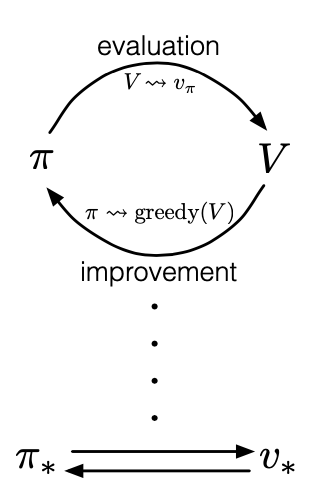
\includegraphics[scale=0.75]{graphics/generalized_policy_iteration.png}
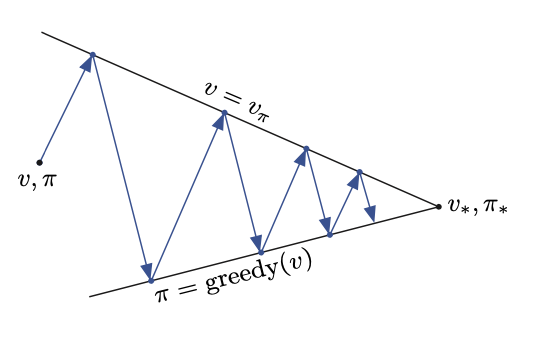
\includegraphics[scale=1]{graphics/generalized_policy_iteration_2.png}
\captionof{figure}{Generalized policy iteration as described in \cite{Sutton1998}.}
\end{minipage}
\end{center}

This generalized policy iteration is one possible solution to the \emph{control problem} (in contrast to the prediction problem), that is the relevant problem of finding a good policy. \\

The policy improvement step is typically done by making the policy $\pi$ greedy with respect to the most recent version of the value function $v$ or action value function $q$. During the project, we relied on an action-value function $q$, since in this case no model of the environment's dynamics is required to construct the greedy policy 

\begin{equation} \label{eq:greedy_policy_update}
	\pi(s) := \argmax_{a \in \mathcal{A}} q(s, a).
\end{equation}

For the evaluation or prediction part of the generalized policy iteration, we relied on on-policy \emph{Temporal Difference} learning. Just like Monte Carlo methods, Temporal Difference methods are model free and allow for learning directly from raw experience without a model of the world. In contrast to Monte Carlo methods, Temporal Difference methods allow for \emph{bootstrapping}, that is, they can update estimates based in part on other learned estimates, without waiting for a final outcome. This was important for the Bomberman example, since the agent should not be forced to wait till the end of a round for an update.

\subsection{Sarsa algorithm}

The first Temporal Difference learning method, we used was the \emph{Sarsa algorithm}, which updates after every transition from a nonterminal state.  \\
\begin{equation} \label{eq:sarsa_update}
	Q(S_t, A_t) \leftarrow Q(S_t, A_t) + \alpha \big[R_{t+1} + \gamma Q(S_{t+1}, A_{t+1}) - Q(S_t, A_t)\big],
\end{equation}
where
\begin{itemize}
	\item $S_t$ denotes the initial state of the state transition,
	\item $A_t$ denotes the action taken in the transition,
	\item $R_{t+1}$ denotes the reward the agent received for the transition.
\end{itemize}
$Q(S_t, A_t)$ denotes the value estimate of the state-action-tuple $(S_t, A_t)$ and is defined to be zero for all tuples $(S_t, A_t)$, where $S_t$ is terminal.
\begin{itemize}
	\item $S_{t+1}$ denotes the state of the agent after the state transition,
	\item $A_{t+1}$ denotes the action the agent will take after the state transition. Note that the value estimation $Q(S_{t+1}, A_{t+1})$ is zero for $S_{t+1}$ terminal, independently of the action $A_{t+1}$. Thus, no action is required for the evaluation of terminal states $S_{t+1}$. 
\end{itemize}
Moreover, this first algorithm introduces two important hyperparameters,
\begin{itemize}
	\item $\alpha > 0$ denotes the \emph{learning rate} and controls the effect of a single 
	\item $\gamma \in [0, 1]$ denotes the \emph{discount factor}, which is a measure for the weight of future rewards. 
\end{itemize}

The update rule uses every element of the quintuple of events, $(S_t, A_t, R_{t+1}$, $S_{t+1}, A_{t+1})$, that make up a transition from one state–action pair to the next. In this way, the quintuple gives rise to the name Sarsa for the algorithm. Sarsa was our initial choice for a learning algorithm since it has excellent convergence properties as proven in \cite{Singh2000} and is easy to implement. \\

From the Sarsa prediction algorithm it is straightforward to construct an on-policy control method using the generalized policy iteration. To do so, we gradually estimate the action-value function $q_\pi$ with the behaviour policy $\pi$ and simultaneously let $\pi$ greedily adapt to $q_\pi$ as in \eqref{eq:greedy_policy_update}. One of the frequently encountered conditions to guarantee the convergence of this iteration, is that all state-action pairs are in theory visited infinitely often. Without doubt, this is not possible in the large state space of the bomberman game. Still, exploration was necessary as easily seen in the classical example of the \emph{exploration-exploitation-tradeoff}. 

\subsection{Exploration-exploitation-tradeoff}
In the beginning of the project, we used $\epsilon$-greedy policies to ensure exploration of unknown action-state combinations. For every policy action-value function $q$ and $\epsilon \in [0, 1]$ the corresponding $\epsilon$-greedy policy selects a random action with probability $\epsilon$ and the action greedily proposed by $q$ with probability $1-\epsilon$. Thus, 

\begin{equation} \label{epsilon-greedy-policy}
	\epsilon\text{-greedy}(q)(s) \sim
\begin{cases}
 	U(\mathcal{A}_s) & X = 1\\
 	\argmax_{a} q(s, a) & X = 0
\end{cases},
\end{equation}
where $U(\mathcal{A}_s)$ denotes the uniform distribution on the set of possible actions in the state $s$ and $X \sim \text{Bin}(1, p)$ denotes a binomially-distributed random variable with success probability $p$. \\

In later stages of the project in which it was necessary for the agent to cautiously drop bombs to complete tasks, exploration with blind tentative $\epsilon$-greedy policies was not practicable anymore. Therefore, we switched to softmax-policies to still guarantee exploration. For every action-value function $q$ and \emph{temperature} $\rho \in (0, \infty)$, the $\rho$-softmax policy selects actions in state $s$ with varying probability according to the corresponding estimated value $q(s, a)$ of the state-action tuple $(s, a)$. To be more precise, 
\begin{equation*}
	\mathbb{P}(\rho\text{-softmax}(q)(s) = a) = \frac{\exp\Big(\frac{q(s, a)}{\rho}\Big)}{\sum_{a_i \in \mathcal{A}_s} \exp\Big(\frac{q(s, a_i)}{\rho}\Big)}.
\end{equation*}
Similar to $\epsilon$ for $\epsilon$-greedy policies, the temperature $\rho$ determines the extent of the probabilistic nature of the corresponding $\rho$-softmax-policy. For $\rho \rightarrow \infty$ the corresponding $\rho$-softmax policy converges to the uniform distribution $U(\mathcal{A}_s)$ on the set of possible actions $\mathcal{A}_s$. For $\rho \rightarrow 0$ the $\rho$-softmax policy selects the action with maximal estimated corresponding value $q(s, a)$ with arbitrarily high probability. \\

% TODO: Ref section.
A more detailed description of our decision-making process regarding the different exploration possibilities can be found in section \ref{}.

\subsection{The tyranny of the single time step}

The Sarsa algorithm performed really well to train some initial agents on the first task. Still, one major drawback of single time step methods are described by Sutton as the \emph{tyranny of the single time step}. The tyranny of the single time step denotes the disadvantage of one-step method, such as Sarsa, that the update of an action and the amount of bootstrapping is linked. It is reasonable to update the action value function frequently to take into account anything that has changed. Unfortunately, bootstrapping works best  over longer time periods in which a significant change in states has occurred. For one step methods the update intervals and bootstrapping time periods are equal and a compromise must be made. To defy the tyranny of the single time step and to enable fast training, we therefore switched to an $n$-step method with bootstrapping over multiple steps.

\subsection{$n$-Step Sarsa}

The simple idea behind $n$-step Sarsa is to modify the update rule \eqref{eq:sarsa_update} to update an earlier estimate based on how it differs from an  estimate \emph{after $n$-step}, instead of based on how it differs from an estimate after a single time step. This gives rise to the new update rule

\begin{equation} \label{eq:n_step_sarsa_update}
	Q(S_t, A_t) \leftarrow Q(S_t, A_t) + \alpha \big[\sum_{i=1}^n \gamma^{i-1}R_{t+i} + \gamma^n Q(S_{t+n}, A_{t+n}) - Q(S_t, A_t)\big].
\end{equation}

The $n$-step Sarsa methods form a family of learning methods. Since Monte Carlo methods perform their update only after every game, they can be considered as an extreme case of $n$-step Sarsa methods with $n = T$, where $T$ denotes the number of steps per game. 

\begin{center}
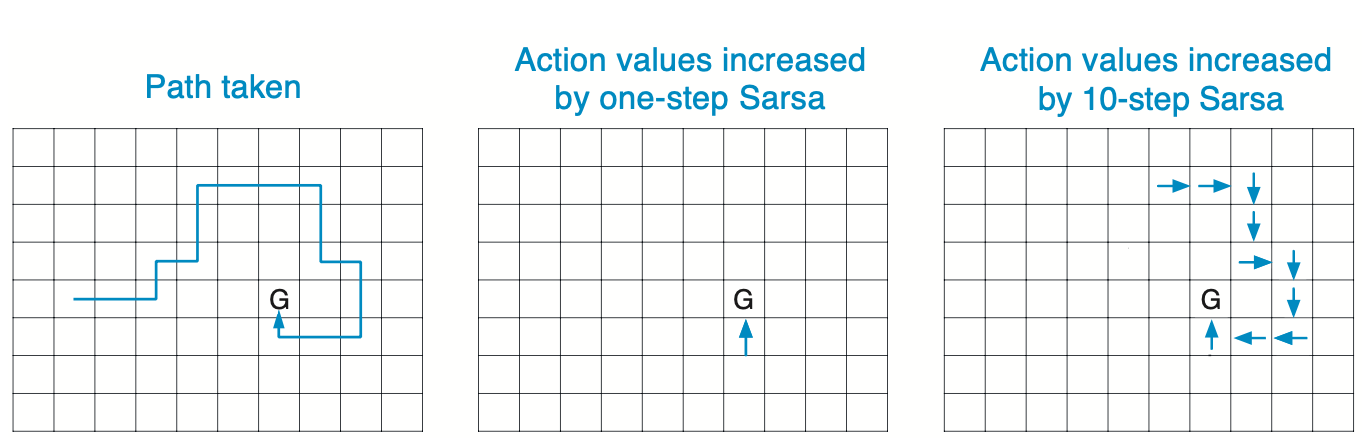
\includegraphics[scale=0.5]{graphics/n_step_sarsa.png}
\end{center}

% TODO: Ref https://arxiv.org/abs/1608.05151

Controlling from which states bootstrapping occurs is important, because it affects the fundamental trade-off between bias and variance of updates. Special motivation for the upgrade of the Sarsa algorithm to the $n$-step Sarsa algorithm was provided by the paper \emph{Effective Multi-step Temporal-Difference Learning for Non-Linear Function Approximation} by \ref{}. We achieved the best training results with an intermediate value of $n$ $(n \approx 4)$, which illustrates how the abstraction of one step Temporal Difference and Monte Carlo methods to $n$-step learning methods can increase the performance of the two extreme methods. The results of our associated simulation study are in line with previous research by Sutton \ref{} and they can be found in section \ref{}. 

\subsection{Learning with eligibility traces}

The last and final update to the learning algorithm was to upgrade the $n$-step Sarsa method to a generalized Sarsa($\lambda$) algorithm. Just like $n$-step Sarsa, this new family of methods unifies Temporal Difference learning and Monte Carlo methods. Sutton describes the $n$-step approach that we have been taking so far as a forward view of a learning algorithm. For every state visited, the update algorithm looks $n$-steps forward in time to all the future rewards and punishments to determine the next update. The Sarsa($\lambda$) methods reverse this view by using a short term memory, which stores information about the recently visited states and updates them accordingly. The results are similar to an $n$-step method, but moreover eligibility traces offer an elegant algorithmic mechanism with significant computational advantages. Instead of storing the last $n$ state transition tuples $(S_t, A_t, S_{t+1}, R_{t+1})$, the Sarsa($\lambda$) algorithm stores an eligibility trace $z$ of dimension $d$. When the action-value function is not approximated by a parametric function $\hat q_{w}$, $d$ is equal to the product of the cardinality of the state space and the cardinality of the action space. This is infeasible for the Bomberman game with large state space. Still, we restrict ourselves to this theoretical case here to provide a clear explanation. In this setting we may index $z$ by a state and an action $z_{s, a}$. $z_{s, a}$ serves as a short-term memory, which measures the weight of the state-action tuple $(s, a)$ on the current state. Computationally, this is done by bumping up the component $z_{s, a}$, whenever the state-action pair $(s, a)$ participates in producing an estimated value, e.g. action $a$ was performed in state $s$. Then, the corresponding component $z_{s, a}$ fades away exponentially in time. When the agent receives a reward, all state action values $q(s, a)$ are updated, but the update is weighted by their corresponding component in $z$. Thus, larger updates will be performed for the tuples $(s, a)$, which were visited just shortly before the reward occurred. 

\begin{center}
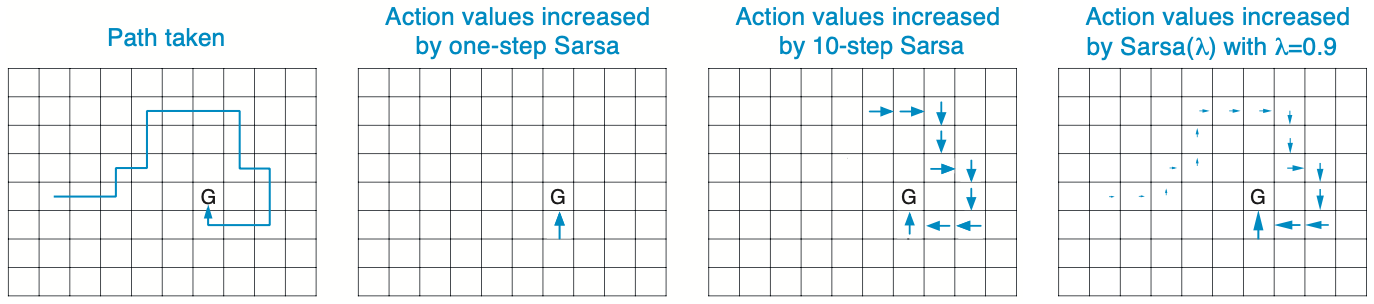
\includegraphics[scale=0.6]{graphics/sarsa_lambda.png}
\end{center}

The hyperparameter $\lambda \in [0, 1]$ determines how fast the components of the eligibility trace $z$ fade away in time. The fading of the components is implemented as a multiplication of $z$ with $\lambda$ in each time step. In the first extreme case $\lambda = 0$, a new reward won't effect the action-value estimation of a state-action pair, which occurred more than a single time step ago. In particular, we have Sarsa(0) = 1-step Sarsa = Sarsa. The second extreme case $\lambda = 1$, yields the well-known Monte Carlo method, again. Thus, the family of learning methods Sarsa($\lambda$) unifies single step Temporal Difference learning and Monte Carlo methods in a continuous way, in contrast to the discrete unification of the two families by $n$-step methods. Moreover, Sarsa(1) is applicable even in infinite non-episodic task, where the standard Monte Carlo method fails, since there is no point in time to perform the update. \\

In our case, the switch from $n$-step Sarsa to the Sarsa($\lambda$) method did neither come with an increased training performance nor with a decreased training performance. Nevertheless, this was not clear beforehand. Sutton for example provides studies in his book, where Sarsa($\lambda$) easily outperforms multi-step methods. In hindsight, we learned a lot while studying the theoretical basis for Sarsa($\lambda$) and our final implementation is much more elegant and straight-forward than the implementation of the $n$-step variant. \\

\section[Action-value function approximation]{Action-value function approximation \hfill \small \normalfont\textit{by Matthias Hericks}}

In the previous section, no assumptions were made about the structure of the action-value function $q$ and we implicitly considered tabular solution methods in their most general form. Because of the large feature space of the Bomberman environment, this is infeasible in practice. For the actual implementation, we had to rely on a parametric action-value function $\hat q_{w} = \hat q(\cdot, w)$ depending on a \emph{weight vector} $w$ of dimension $d \ll |\mathcal{S}|$. Therefore, a change in the weight vector potentially effects the estimation of the value of many different action-state tuples. \\

Fortunately, all of the learning methods presented in the last section can easily be modified to update the weights of a parametric action-value function. Generally, the weight update can be written as
\begin{equation} \label{eq:general_weight_update}
	w_{t+1} \leftarrow w_t + \alpha \big[U_t - \hat q(S_t, A_t, w_t)\big]\nabla \hat q(S_t, A_t, w_t),
\end{equation}
where $\nabla \hat q$ denotes the gradient of $\hat q$ with respect to $w$ and $U_t$ denotes the \emph{update target} that $s$’s estimated value is shifted toward. In the Sarsa algorithm, the update target $U_t$ is defined as $R_{t+1} + \gamma \hat q(S_{t+1}, A_{t+1}, w_{t})$. Using this definition of the update target \ref{eq:general_weight_update} becomes
\begin{equation*}
	w_{t+1} \leftarrow w_t + \alpha \big[R_{t+1} + \gamma \hat q(S_{t+1}, A_{t+1}, w_t) - \hat q(S_t, A_t, w_t)\big]\nabla \hat q(S_t, A_t, w_t),
\end{equation*}
which nearly resembles the Sarsa update in \eqref{eq:sarsa_update}. Moreover, we modified the $n$-step Sarsa update as well as the Sarsa($\lambda$) methods accordingly. \\

\subsection{Linear function approximation}

More concretely, we began with a simple linear function approximation, that is we write
\begin{equation*}
	\hat q(s, a, w) = w(a)^T \cdot x(s) = \sum_{i=1}^d x(s)_i w(a)_i,
\end{equation*}
where
% TODO: Ref chapter.
\begin{itemize}
	\item $x(s)$ denotes a $d$-dimensional feature vector extracted from the game state $s$ (see Chapter \ref{}), 
	\item $w(a)$ is a weight vector for every possible action $a$.
\end{itemize}
In this section, we have to ensure that \eqref{eq:general_weight_update} only updates the weights $w(A_t)$ for the specific action taken. \\

% TODO: Find proof.
The advantage of using a linear function approximator is its simple form as well as the excellent convergence properties proven in \ref{}. This linear function approximation was sufficient for many different tasks. The disadvantage is the need for \emph{good} features $x(s)$. In the end, we sticked with this linear model and tried to increase the quality of the model by crafting high-quality features by hand as well as with the help of a genetic algorithm for feature extraction. 







